\documentclass[a4paper,UTF8]{article}
\usepackage{ctex}
\usepackage[margin=1.25in]{geometry}
\usepackage{color}
\usepackage{graphicx}
\usepackage{amssymb}
\usepackage{amsmath}
\usepackage{amsthm}
\usepackage{enumerate}
\usepackage{bm}
\usepackage{hyperref}
\usepackage{epsfig}
\usepackage{color}
\usepackage{mdframed}
\usepackage{lipsum}
\usepackage{mathtools}
\usepackage{hyperref}
\usepackage{diagbox}
\usepackage{float}
\usepackage{caption}
\usepackage{algorithm}
\usepackage{algorithmicx}  
\usepackage{algpseudocode}
\usepackage{amsmath} 
\usepackage{graphicx}
\usepackage{subfigure}
\usepackage{url}
\newmdtheoremenv{thm-box}{myThm}
\newmdtheoremenv{prop-box}{Proposition}
\newmdtheoremenv{def-box}{定义}
\usepackage{listings}
\usepackage{xcolor}
\lstset{
	numbers=left, 
	numberstyle= \tiny, 
	keywordstyle= \color{ blue!70},
	commentstyle= \color{red!50!green!50!blue!50}, 
	frame=shadowbox, % 阴影效果
	rulesepcolor= \color{ red!20!green!20!blue!20} ,
	escapeinside=``, % 英文分号中可写入中文
	xleftmargin=2em,xrightmargin=2em, aboveskip=1em,
	framexleftmargin=2em
} 

\usepackage{booktabs}

\setlength{\evensidemargin}{.25in}
\setlength{\textwidth}{6in}
\setlength{\topmargin}{-0.5in}
\setlength{\topmargin}{-0.5in}

% \setlength{\textheight}{9.5in}
%%%%%%%%%%%%%%%%%%此处用于设置页眉页脚%%%%%%%%%%%%%%%%%%
\usepackage{fancyhdr}                                
\usepackage{lastpage}                                           
\usepackage{layout}                                             
\footskip = 10pt 
\pagestyle{fancy}                    % 设置页眉                 
\lhead{研一下学期}                    
\chead{论文阅读笔记}                                                
% \rhead{第\thepage/\pageref{LastPage}页} 
\rhead{Step7}                                                                                               
\cfoot{\thepage}                                                
\renewcommand{\headrulewidth}{1pt}  			%页眉线宽,设为0可以去页眉线
\setlength{\skip\footins}{0.5cm}    			%脚注与正文的距离           
\renewcommand{\footrulewidth}{0pt}  			%页脚线宽,设为0可以去页脚线

\makeatletter 									%设置双线页眉                                        
\def\headrule{{\if@fancyplain\let\headrulewidth\plainheadrulewidth\fi%
\hrule\@height 1.0pt \@width\headwidth\vskip1pt	%上面线为1pt粗  
\hrule\@height 0.5pt\@width\headwidth  			%下面0.5pt粗            
\vskip-2\headrulewidth\vskip-1pt}      			%两条线的距离1pt        
 \vspace{6mm}}     								%双线与下面正文之间的垂直间距              
\makeatother  

%%%%%%%%%%%%%%%%%%%%%%%%%%%%%%%%%%%%%%%%%%%%%%
\numberwithin{equation}{section}
%\usepackage[thmmarks, amsmath, thref]{ntheorem}
\newtheorem{theorem}{Theorem}
\newtheorem*{definition}{Definition}
\newtheorem*{solution}{Solution}
\newtheorem*{prove}{Proof}
\newcommand{\indep}{\rotatebox[origin=c]{90}{$\models$}}

\usepackage{multirow}

%--

%--
\begin{document}
\title{论文阅读笔记\\
Step7}
\author{MF1833063, 史鹏, spwannasing@gmail.com}
\maketitle

\newpage
\section{Answering while Summarizing:Multi-task Learning for Multi-hop QA with Evidence Extraction}
本文基于HotpotQA,提出了一个叫Query Focused Extractor (QFE)的模型,基于 extractive summarization模型,另外相比已有的模型,克服了预测evidence sentence之间相互独立的问题(通过使用RNN),以及引入了Multi-Task,
可以和任意的RC模型结合。亮点是即使QFE和一个简单的baseline RC模型结合起来,也能达到evidence extraction score上的SOTA效果。
\begin{figure}[H]
	\centering
	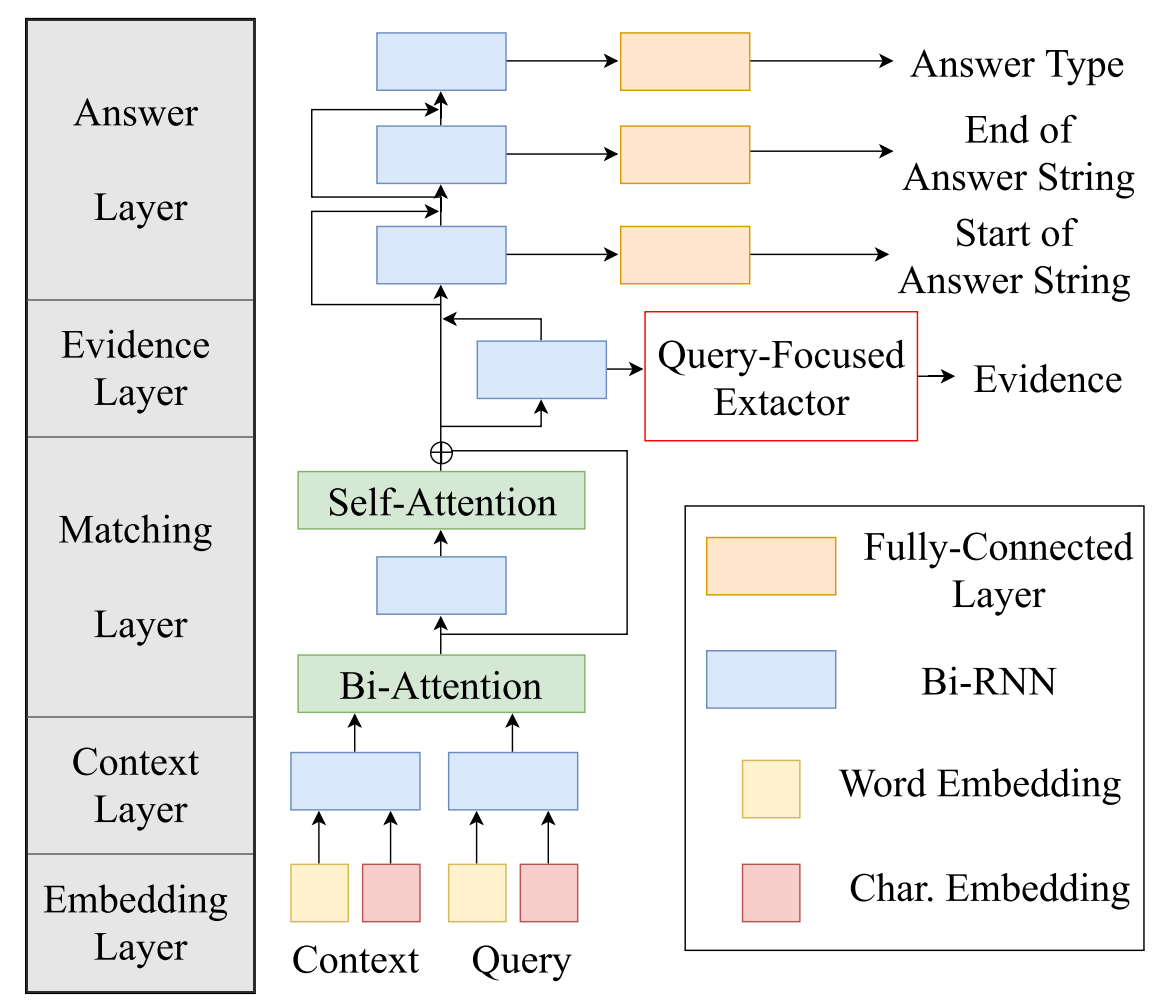
\includegraphics[width=0.6\textwidth]{1-1.png}
\end{figure}
\begin{figure}[H]
	\centering
	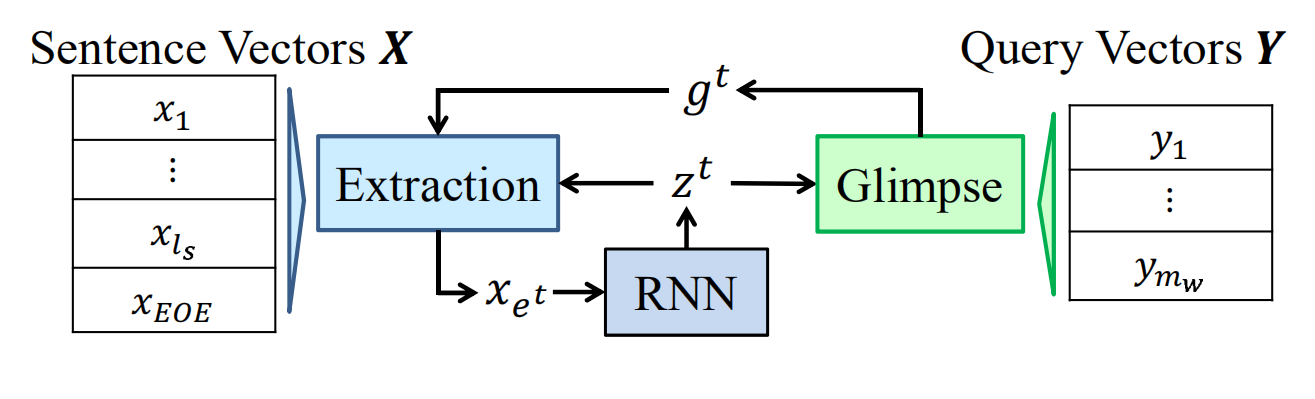
\includegraphics[width=0.6\textwidth]{1-2.png}
\end{figure}
\begin{equation}
	z^{t}=\mathrm{R} \mathrm{NN}\left(z^{t-1}, x_{e^{t}}\right) \in \mathbb{R}^{2 d_{c}}
	\end{equation}

	\begin{equation}
		\operatorname{Pr}\left(i ; E^{t-1}\right)=\operatorname{softmax}_{i}\left(u_{i}^{t}\right)
		\end{equation}
		\begin{equation}
		u_{i}^{t}=\left\{\begin{array}{ll}{v_{p}^{\top} \tanh \left(W_{p 1} x_{i}+W_{p 2} g^{t}+W_{p 3} z^{t}\right)} \\ {} & {\left(i \notin E^{t-1}\right)} \\ {-\infty} & {(\text { otherwise })}\end{array}\right.
		\end{equation}

	\begin{equation}
	\begin{aligned} g^{t} &=\sum_{j} \alpha_{j}^{t} W_{g 1} 1_{j} \in \mathbb{R}^{2 d_{c}} \\ \alpha^{t} &=\operatorname{softmax}\left(a^{t}\right) \in \mathbb{R}^{m_{w}} \\ a_{j}^{t} &=v_{g}^{\top} \tanh \left(W_{g 1} y_{j}+W_{g 2} z^{t}\right) \end{aligned}
	\end{equation}
	\begin{equation}
	\begin{aligned} L_{E}=-\sum_{t=1}^{|E|} & \log \left(\max _{i \in E \backslash E^{t-1}} \operatorname{Pr}\left(i ; E^{t-1}\right)\right) \\ &+\sum_{i} \min \left(c_{i}^{t}, \alpha_{i}^{t}\right) \end{aligned}
	\end{equation}
	\begin{equation}
		L=L_{A}+L_{E}
		\end{equation}

\newpage
\section{Do you know that Florence is packed with visitors?Evaluating state-of-the-art models of speaker commitment}
这篇论文展示出了带有语言学知识的模型的巨大潜力

对基于规则的和双向LSTM这两种最先进的说话人承诺模型进行了系统的评价

论文中的语言学分析给人启发,也展现出了系统的优势和劣势

当一个人,比如 Mary,问你「你知不知道佛罗伦萨全都是游客?」,我们会认为她相信佛罗伦萨全都是游客;但如果她问「你觉得佛罗伦萨游客多吗?」,我们就不会这样认为。推断说话人承诺(或者说事件真实度)是问答和信息提取任务中的关键部分。在这篇论文中,作者们探索了这样一个假说:语言学信息的缺乏会影响说话人承诺模型中的错误模式。他们的验证方式是在一个有挑战性的自然语言数据集上分析模型错误的语言学关联性。作者们在 CommitmentBank 这个由自然英语对话组成的数据集上评价了两个目前最好的说话人承诺模型。CommitmentBank 数据集已经经过了说话人承诺标注,方式是在 4 种取消蕴含的环境中向着时态嵌入动词(比如知道、认为)的补充内容进行标注。作者们发现,一个带有语言学知识的模型能展现比基于 LSTM 的模型更好的表现,这表明如果想要在这样的有挑战性的自然语言数据中捕捉这些信息的话,语言学知识是必不可少的。对语言学特征的逐项分析展现出了不对称的错误模式:虽然模型能在某些状况下得到好的表现(比如否定式),但它很难泛化到更丰富的自然语言的语言学结构中(比如条件句式),这表明还有很大提升的空间。

\begin{figure}[H]
	\centering
	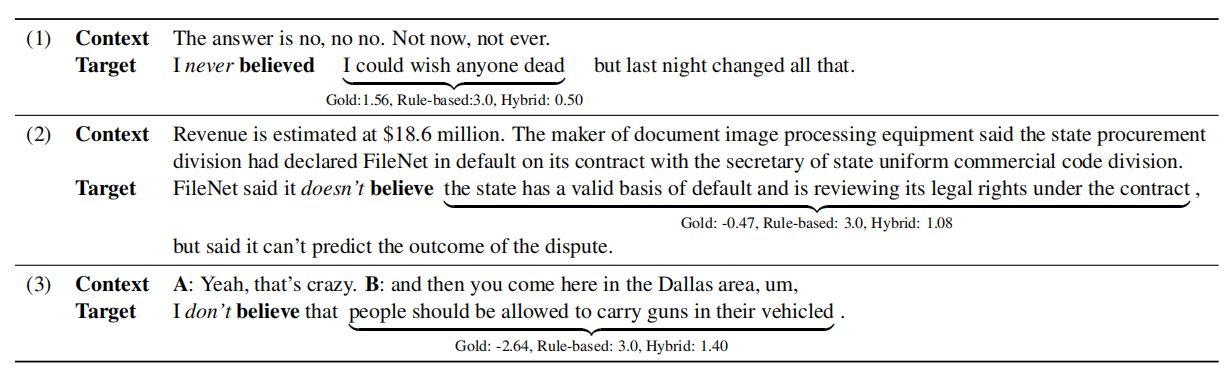
\includegraphics[width=\textwidth]{2-1.png}
\end{figure}

\newpage
\section{Emotion-Cause Pair Extraction:A New Task to Emotion Analysis in Texts}
情绪原因提取(Emotion cause extraction ,ECE)是一项旨在提取文本中某些情绪背后潜在原因的任务,近年来由于其广泛的应用而受到了很多关注。然而,它有两个缺点:1)情绪必须在ECE原因提取之前进行标注,这极大地限制了它在现实场景中的应用;2)先标注情绪然后提取原因的方式忽略了它们是相互指示的事实。

\end{document}